Stružnica je najstarejši obdelovalni stroj,
ki se ga uporablja pri struženju. Še vedno se
veliko uporablja v strojništvu in lesarstvu,
tako da skoraj ni delavnice brez tega obdelovalnega stroja.
Za razliko od rezkalnih strojev glavno krožno gibanje opravlja
obdelovanec, zato se največkrat na stružnici obdelujejo rotacijsko
simetrični kosi. Obdelujejo se lahko tudi rotacijsko nesimetrični kosi,
vendar zanje potrebujemo posebno vpetje, obdelana površina pa je
vedno vzporedna z osjo rotacije.

\noindent Glavni deli standardne stružnice so:
\begin{itemize}
	\item postelja,
	\item vretenjak,
	\item podajalni menjalnik,
	\item sani s suporti,
	\item konjiček,
	\item lineta.
\end{itemize}

Prikazani so na spodnji Sliki \ref{img:deli_struznice} na primeru univerzalne klasične stružnice.
\begin{figure}[H]
	\begin{center}
		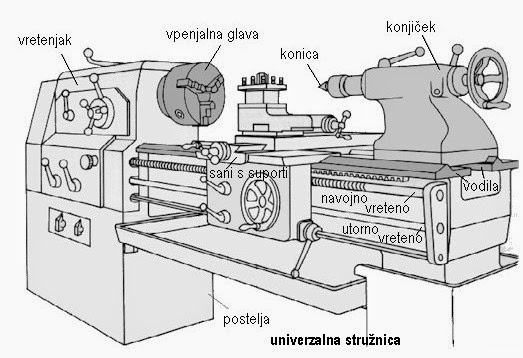
\includegraphics[width=10cm]{deli_struznice.jpg}
		\caption{Glavni deli stružnice
			\cite{deli_struznice}}
		\label{img:deli_struznice}
	\end{center}
\end{figure}

\noindent Glede na glavne dele in njihovo orientacijo ter namestitev razlikujemo
predvsem naslednje vrste stružnic:
\begin{itemize}
	\item univerzalna stružnica,
	\item čelna stružnica,
	\item karoselna stružnica,
	\item revolverska stružnica.
\end{itemize}

\noindent Iz navedenih oblik pa so se razvile še posebej specializirane
stružnice, kot na primer:
\begin{itemize}
	\item kopirna ali podstružilna stružnica,
	\item avtomatska stružnica,
	\item numerično krmiljena stružnica (ali krajše CNC-stružnica).
\end{itemize}

\subsection{Struženje}
''Struženje je najbolj razširjen postopek odrezavanja za
obdelavo valjastih obdelovancev, možno pa je stružiti tudi ravne ploskve
in celo nekatere neokrogle oblike, če orodje med delom niha sinhronizirano
z vrtenjem obdelovanca.'' \cite{sts_arhiv_struzenje}

Glavno gibanje pri struženju je rotacijsko in ga opravlja
obdelovanec. Podajalno gibanje je navadno premočrtno ali pa
sledi poljubni krivulji. Struženje zavzema velik delež celotne
obdelave z odrezavanjem, zato je struženje najnatančneje
raziskan postopek. Raziskovanja pri struženju so dala vrsto
zakonitosti, ki so osnove za vse postopke odrezavanje kovin.

Poznamo vzdolžno -- Slika \ref{vzdolzno_struzenje},
prečno -- Slika \ref{precno_struzenje}, stožčasto, profilno,
zarezno struženje -- Slika \ref{struzenje_utora}, kot tudi
struženje navoja, podstruževanje za izdelavo neokroglih
oblik in kopirno struženje, kjer se izdeluje kompleksnejše oblike.

\begin{figure}[H]
	\begin{center}
		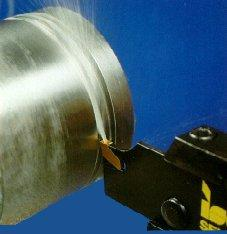
\includegraphics[width=8cm]{struzenje_utora.jpg}
		\caption{Struženje utora
			\cite{sts_arhiv_struzenje}}
		\label{struzenje_utora}
	\end{center}
\end{figure}

\begin{figure}[H]
	\begin{center}
		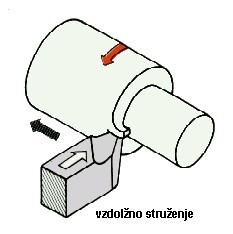
\includegraphics[width=8cm]{vzdolzno_struzenje.jpg}
		\caption{Vzdolžno struženje
			\cite{sts_arhiv_struzenje}}
		\label{vzdolzno_struzenje}
	\end{center}
\end{figure}

\begin{figure}[H]
	\begin{center}
		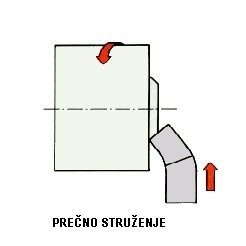
\includegraphics[width=8cm]{precno_struzenje.jpg}
		\caption{Prečno struženje
			\cite{sts_arhiv_struzenje}}
		\label{precno_struzenje}
	\end{center}
\end{figure}

\subsubsection{Orodje pri struženju}
Orodja pri struženju so sestavljena iz rezila in držača. Rezilo je
iz tršega materiala, specializiranega za odrezovanje, medtem ko je
držač iz cenejšega konstrukcijskega ali poboljšanega jekla.
Rezilo je lahko na držač mehansko pritrjeno ali pa prilotano.
Celoten držač je pritrjen na stružnico s posebnim
vpetjem na prečnem suportu. Nekatera vpetja omogočajo tudi nastavitev
višine in kota rezalnega orodja.

Včasih se je veliko več uporabljalo nalotane nože z rezilom iz
karbidnih trdnin. Na Sliki \ref{karbidni_nozi} je prikazana večina
standardnih oblik karbidnih nožev za zunanje struženje.
Danes se največkrat uporablja nože z obračalnimi ploščicami,
ki se veliko lažje zamenjajo in zdržijo tudi veliko več obrabe.
Obračalne ploščice so sestavljene iz raznih materialov, največkrat
so sintrane in nato prevlečene s tršimi sloji, odpornimi na obrabo.
So specializirane za različne materiale, pred uporabo pa moramo
dobro premisliti, katero bomo uporabili.

\begin{figure}
	\begin{center}
		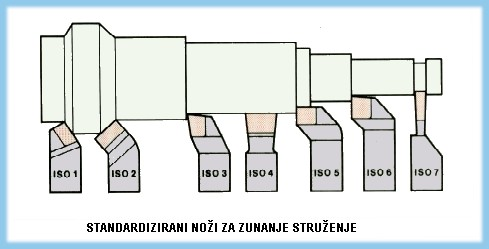
\includegraphics[width=8cm]{karbidni_nozi.jpg}
		\caption{Standardni karbidni noži za zunanje struženje
			\cite{sts_arhiv_struzenje_karbidni_nozi}}
		\label{karbidni_nozi}
	\end{center}
\end{figure}

\begin{figure}
	\begin{center}
		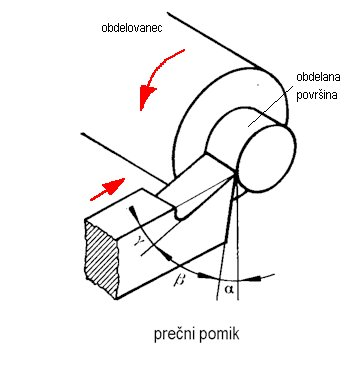
\includegraphics[width=4cm]{rezalni_koti.jpg}
		\caption{Koti rezalnih robov na orodju
			\cite{sts_arhiv_struzenje_rezalni_koti}}
		\label{rezalni_koti}
	\end{center}
\end{figure}

Pomembna je tudi oblika samega rezalnega roba. Nepravilna
oblika lahko privede do veliko hitrejše obrabe orodja kot tudi
do slabe površinske obdelave. Na Sliki \ref{rezalni_koti} so narisani
pomembni koti za geometrijo orodja. Kot \(\gamma\) je cepilni kot in prispeva
k zmanjšanju rezalne sile. Če je ta prevelik, potem je orodje veliko
šibkejše in manj trdno. Prosti kot \(\alpha\) pa mora biti dovolj velik,
da pri struženju ne pride do drsenja proste ploskve po površini, a
moramo paziti, saj lahko enako kot pri kotu \(\gamma\) pride do oslabitve
trdnosti orodja.

\subsubsection{Vrtanje}
Je operacija obdelave materiala z odrezovanjem.
Pri vrtanju se lahko vrti orodje, obdelovanec ali oba hkrati,
pri čemer za izračun pomika vrtljaje seštevamo, če se ti vrtijo
v nasprotno smer. Rezultat operacije je izvrtina valjaste oblike.
Vrtamo z svedri, ki imajo za vsak material določen rezni kot in kot vzpona
vijačnice. Npr. za medenino je kot vzpona zelo velik, da se
krhki ostružki hitro odstranijo iz luknje. Za jekla, kjer so
ostružki največkrat dolgi in nepretrgani, uporabljamo svedre z
zelo majhnim kotom vzpona.

Svedri za kovino so večinoma trdokovinski ali pa narejeni iz
hitroreznega jekla in prevlečeni s titanovo zlitino.
Naziv »spiralni sveder« ki se ponekod še uporablja, je napačen.
Spirala je krivulja na ravnini, medtem ko je vijačnica krivulja
skozi prostor okoli osi, zato bi praviloma morali uporabljati
izraz vijačni sveder.
Poznamo še lasersko vrtanje, ki se uveljavlja v zahtevnih
proizvodnjah, kjer je potrebno izdelati zelo majhne luknje,
60-- 50 µm, kar s svedri ni mogoče. Lasersko vrtanje pa je zelo
uporabno tudi pri vrtanju poševnih izvrtin, kar je za običajno
vrtanje velik izziv.
Obstajajo še elektroerozijske prebijalke, ki lahko z bakrenimi ali
grafitnimi elektrodami prebijejo le elektroprevodne materiale.

Za primer imamo spodaj na Sliki \ref{hss_sveder} prikazan navaden
vijačni HSS-sveder, prevlečen s titanovo zlitino.
\begin{figure}[H]
	\begin{center}
		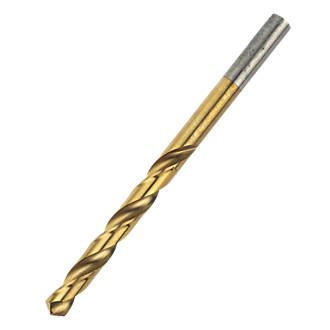
\includegraphics[width=8cm]{sveder.jpg}
		\caption{Navaden HSS-sveder
			\cite{sveder}}
		\label{hss_sveder}
	\end{center}
\end{figure}
\subsubsection{Povrtavanje}
Je operacija vrtanja, katere namen je izboljšanje točnosti in
hrapavosti površine v že narejeni izvrtini. Največkrat se
uporablja, ko imamo ujem in moramo doseči gladko površino v
mejah natančnosti od IT6 do IT11. Orodja za povrtavanje, povrtala,
imajo 6 ali več rezil. Na spodnji Sliki \ref{povrtalo} lahko vidimo
primer ročnega povrtala s šestimi rezili, ki se uporablja na
univerzalni stružnici.
\begin{figure}[H]
	\begin{center}
		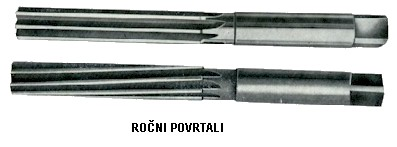
\includegraphics[width=10cm]{povrtalo.jpg}
		\caption{Povrtalo
			\cite{sts_arhiv}}
		\label{povrtalo}
	\end{center}
\end{figure}

\subsubsection{Vrezovanje navoja}
Posebna oblika povrtavanja je vrezovanje navoja. Ta operacija se
lahko izvede samo takrat, ko imamo že predvrtano pravilno
velikost luknje za dani navoj. Orodja za vrezovanje navojev se
imenujejo navojni svedri in so prikazani na spodnji Sliki \ref{navojni_sveder}.
\begin{figure}[H]
	\begin{center}
		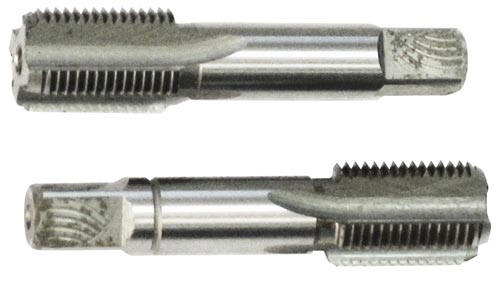
\includegraphics[width=8cm]{navojni.jpg}
		\caption{Navojni sveder
			\cite{sts_arhiv}}
		\label{navojni_sveder}
	\end{center}
\end{figure}
Ta operacija je še posebej zahtevna pri kateri koli vrsti obdelave,
saj je za vrezovanje navoja potreben velik navor kot tudi zelo natančna
sinhronizacija med glavnim in podajalnim gibanjem. Pri struženju
na univerzalni stružnici to največkrat ni problem, saj se lahko navojni
sveder vpne v konjička, ki se nato prosto pomika po vodilih.
Pri izdelavi navoja na CNC-strojih pa moramo paziti, da pravilno vpišemo
obrate in pomike ali pa uporabimo kompenzacijsko glavo, v katero se
vpne navojni sveder, pri čemer nam ta glava omogoča premikanje svedra, če
ne moremo točno uskladiti obratov in pomikov, npr. pri starejših
strojih.

Na stružnih avtomatih, kjer so obrati glavnega vretena navadno konstantni
in tudi navadno ne moremo obrniti smeri vrtenja, uporabimo trik, pri katerem
spreminjamo hitrost vrtenja navojnega svedra. Če imamo 2000 \(\frac{obr}{min}\)
na glavnem vretenu in 2200 \(\frac{obr}{min}\) v nasprotnem vretenu, kamor je
vpet navojni sveder, se ti obrati odštejejo in izgleda, kot da vrezujemo
navoj samo z 200 \(\frac{obr}{min}\). Ko pa hočemo navojni sveder izvleči, samo
zmanjšamo hitrost na nasprotnemu vretenu na npr. 1600 \(\frac{obr}{min}\),
in ker se to vrti počasnejše od glavnega, lahko sveder izvlečemo iz navoja.

\subsubsection{Grezenje}
Je postopek širjenja že obstoječe (nekaj manjka). Orodja imenujemo grezila,
ki vrtajo kvalitetnejšo luknjo kot sveder ali pa pripravlja
luknjo za povrtavanje. Z grezili dosegamo natančnosti luknje od
IT8 do IT10. Poznamo tri vrste grezenja: grobo, fino in oblikovno grezenje.

Za grobo grezenje se največkrat uporablja samo navadni vijačni
sveder, za fino grezenje uporabljmao grezila, za oblikovno grezenje
pa uporabljamo razna stožčasta enorezilna ali večrezilna grezila
za oblikovanje izvrtin.

Spodaj na Sliki \ref{grezilo} je prikazan primer grezenja
luknje za vijak s konusno glavo.

\begin{figure}[H]
	\begin{center}
		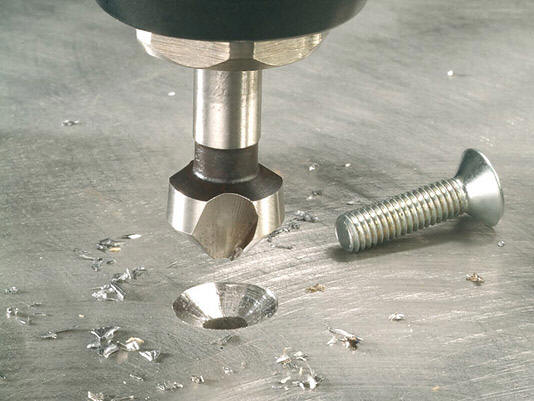
\includegraphics[width=4cm]{grezenje.jpg}
		\caption{Primer grezenja luknje za skritje vijaka
			\cite{sts_arhiv_grezenje}}
		\label{grezilo}
	\end{center}
\end{figure}